\documentclass[10pt]{article}
\usepackage[utf8]{inputenc}
\usepackage{geometry}
\geometry{a4paper, margin=0.6in}
\usepackage{amsmath, amssymb}
\usepackage{enumitem}
\setlist[itemize]{leftmargin=*, itemsep=0pt, topsep=2pt}
\usepackage{natbib}
\bibliographystyle{plain}
\usepackage{tikz}
\usepackage{parskip}
\setlength{\parindent}{0pt}
\usepackage{parskip}
\usepackage{microtype}
\usepackage{times}
\usepackage{float}
\usepackage{graphicx}
\usepackage{subcaption}
\begin{document}

\begin{center}
    \textbf{\large Reinforcement Learning for Optimizing Manipulator Morphology} \\
    \vspace{2pt}
    \textit{Optimizing manipulator morphology (number of joints, link lengths, etc.) using RL with MuJoCo simulation and RRT motion planning.}
\end{center}

\vspace{-5pt}
\section*{Problem \& Why Now}
The premise is that generalized manipulators are expensive, difficult to get around, and not as good at specific tasks as a specialized robot is.
If you can easily design and fabricate a specialized manipulator for the specific tasks you need to automate then it would be more efficient.
RL comes in for the design part.
RL is useful here because it can be used for sparse and nonimmediate rewards like you would expect in a scenario where the reward is completing a task like getting a box from one point to another.
Fast simulation and proven RL algorithms allow for rapid iteration.

\vspace{-5pt}
\section*{Method Sketch}
Grok suggested PPO, I don't know a lot about it at the moment so that is subject to change. 
A PPO agent optimizes morphology parameters: number of joints (discrete, 3--7) and link lengths (continuous, [0.1, 1.0]m). 
For each morphology, RRT plans a path in MuJoCo to push a box to a target, with reward 1 if successful (box within 0.1m), else 0. 
It also might be beneficial to incorporate some kind of distance based reward to increase the density or immediacy of rewards. 
Baselines: (1) RRT on fixed 4-joint arm, (2) BC on expert RRT trajectories.

\begin{figure}[H]
  \centering
  \begin{subfigure}[b]{0.45\textwidth}
    \centering
    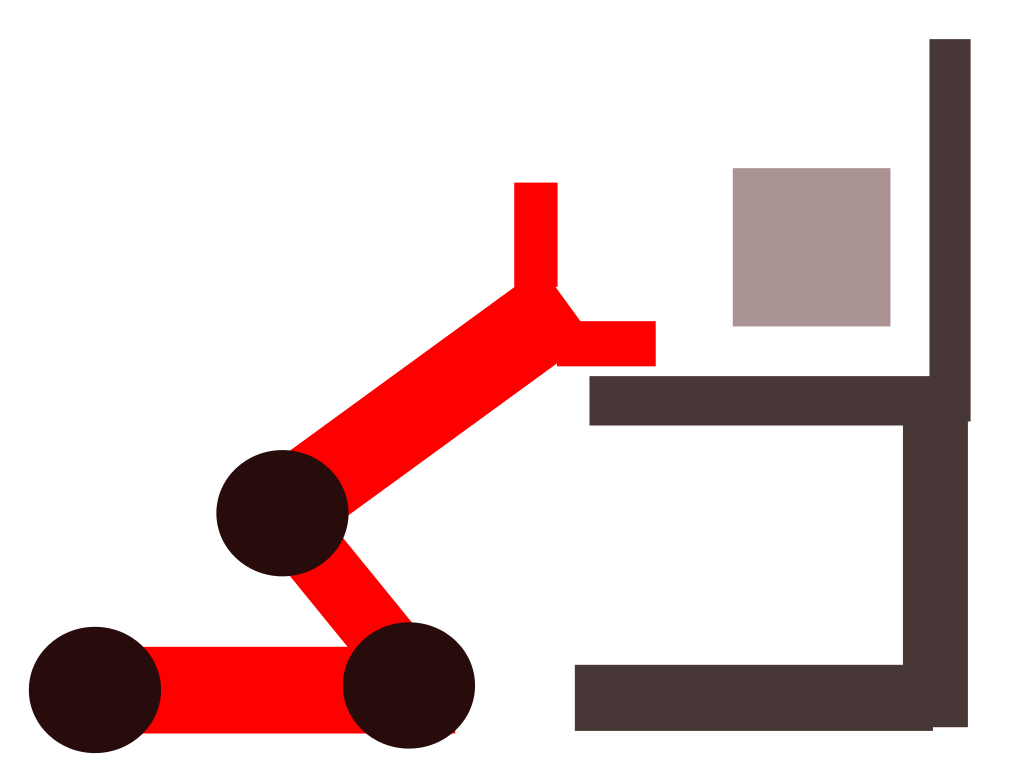
\includegraphics[width=\textwidth]{3link.png}
  \end{subfigure}
  \hfill
  \begin{subfigure}[b]{0.45\textwidth}
    \centering
    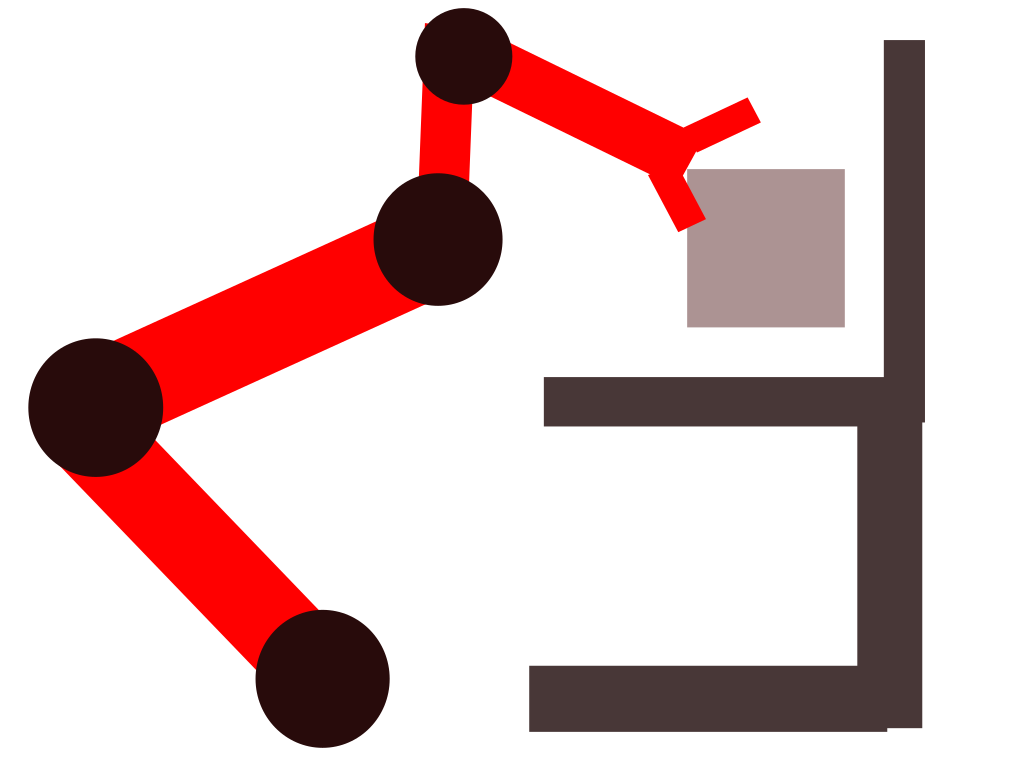
\includegraphics[width=\textwidth]{4link.png}
  \end{subfigure}
  \caption{Varying Link Number/Length}
  \label{fig:varyManFigure}
\end{figure}

\vspace{-5pt}
\section*{Setup}
\textbf{Env/Dataset:} Pytorch for the RL model, MuJoCo for the sim, motion.planning for RRT.
Something like a 5x5x5m environment with a 0.5m cube box, 0.5m cube goal, and 0-2 obstacles.
Observation: joint count, lengths, box/goal positions.
Action: morphology parameters.
Reward: box ending within 0.1m of goal.
Baseline: fixed 4-joint RRT trajectory dataset (self-generated).

\vspace{-5pt}
\section*{Metrics}
\begin{itemize}
    \item \textbf{Primary:} Success rate (box within 0.1m of goal).
    \item \textbf{Secondary:} Sample efficiency (episodes to 60\% success), generalization (test 6--7 joints, new obstacles), RRT planning time.
    \item \textbf{Constraints:} Torque limits, no sim crashes.
\end{itemize}

\vspace{-5pt}
\section*{Feasibility \& Risks}
\textbf{Compute:} LLM approximations: MuJoCo (~50k steps/sec, CPU), RRT (~0.1--1s/plan), PPO (~1000 episodes) runs in $<$10h on RTX 3060. \textbf{Risks:} (1) MJCF errors—validate XML, constrain params. (2) Sparse rewards. \textbf{Mitigation:} Fixed seeds, log episodes/time, share code. No human data/hardware risks.

\vspace{-5pt}
\section*{References}
Initial references just to learn about PPO, RRT, MuJoCo, and BC respectively.
Subject to change.
\begin{thebibliography}{1}
    \bibitem{ppo} Schulman, J., et al. (2017). Proximal Policy Optimization Algorithms. \textit{arXiv:1707.06347}.
    \bibitem{rrt} LaValle, S. M. (2001). Rapidly-Exploring Random Trees: Progress and Prospects. \textit{Algorithmic and Computational Robotics}.
    \bibitem{mujoco} Todorov, E., et al. (2012). MuJoCo: A Physics Engine for Model-Based Control. \textit{IROS}.
    \bibitem{robomimic} Gupta, A., et al. (2021). robomimic: A Framework for Robot Learning from Demonstration. \textit{CoRL}.
\end{thebibliography}

\end{document}